\chapter{Tổng quan về tự động hóa hệ thống}

\newpage
\clearpage

\section{Lý do cần tự động hóa hệ thống}
Không phải ai cũng biết rằng, công việc của quản trị hệ thống thường xoay quanh một loạt các nhiệm vụ lặp đi lặp lại: cấu hình máy chủ, tạo người dùng, quản lý ứng dụng, dịch vụ và các chương trình chạy nền khác. Những công việc này thường được lặp đi lặp lại nhiều lần trong vòng đời của một máy chủ, từ lúc xây dựng hệ thống đến khi ngừng hoạt động. Nó bao gồm cả những việc như quản lý cấu hình trên nhiều cụm máy chủ khác nhau, đồng bộ hóa cấu hình giữa chúng theo chức năng; triển khai backend cho các sản phẩm; triển khai các sản phẩm trên các cụm máy chủ dịch vụ; dọn rác khi đĩa đầy, xóa log không dùng đến, xóa cache ... và đôi lúc là dọn "rác" của những người tiền nhiệm.

\newpage
\clearpage

\section{Các vấn đề nảy sinh}
\begin{itemize}
\item Quản trị hệ thống họ cũng là con người, họ có những vấn đề của con người\footnote{\url{http://en.wikipedia.org/wiki/Human_reliability}}. Điều nghiêm trọng nhất là quên và nhớ.

Một người quản trị hệ thống cho dù giỏi đến đâu cũng có sẽ có lúc quên chính xác những gì mình làm ở trong hệ thống của mình. Nhất là khi rất nhiều người cùng quản trị một hệ thống, mà hệ thống đó lại không được quản lý tốt. Đó là sẽ một vũng lầy!

\item Khi hệ thống đã là một vũng lầy, trên thực tế người ta sẽ đành chấp nhận nó. Nhưng sau một quá trình "chịu đựng", người ta sẽ tính đến chuyện đập đi làm lại, hay còn gọi là "migration". Cách giải quyết ở trong giai đoạn này thường chỉ mang tính chấp vá.

\end{itemize}

\newpage
\clearpage

\section{Cách giải quyết vấn đề}
\begin{itemize}
\item \textbf{Chuẩn hóa quy trình làm việc}

Điển hỉnh là các công ty Nhật, họ có một quy trình làm việc cực kì chặt chẽ, mọi thay đổi đều phải có quy trình và được kiểm soát nghiêm ngặt. Siết chặt các công đoạn làm việc, lịch sử thay đổi và công tác quản lý có thể sẽ hữu ích để giữ cho system không bị rối và luôn chạy ổn định.

\item \textbf{Chấp nhận sống trong "vũng lầy"}. 

Một điều đáng ngạc nhiên là có rất nhiều công ty, tập đoàn từ công nghệ đến cả tài chính trên thế giới phải làm kiểu này. Hệ thống vẫn hoạt động được và vẫn kiếm ra của cải, rất khó để có thể đưa một thay đổi đáng kể nào vào hệ thống đó. Người ta lúc này buộc lòng phải chấp nhận sống trong "vũng lầy"

\item \textbf{Tự động hóa hệ thống}

Đây là hướng mà đồ án này nói tới. Tuy việc tự động hóa hệ thống này đã được ứng dụng rộng rãi từ lâu nhưng nó vẫn là tập hợp của những công nghệ bleeding-edge\footnote{\url{http://en.wikipedia.org/wiki/Bleeding_edge_technology}}. Vì thế theo quan điểm của người viết đồ án thì nó chỉ phù hợp với các công ty công nghệ mà thôi.

\end{itemize}

\newpage
\clearpage

\section{Sự cần thiết của các công cụ quản lý}

Như đã nói ở trên, người quản trị hệ thống với những công việc lặp đi lặp lại này, điều thường thấy là người quản trị hệ thống sẽ cố gắng để tự động hóa chúng bằng các kịch bản (script) và các công cụ. Điều này dẫn đến sự phát triển của các ứng dụng và kịch bản tùy chỉnh. Những kịch bản này thường phức tạp, không có tài liệu đi kèm, và chỉ hoạt động trên một số hệ thống nhất định.

Việc này không có gì độc đáo cả, và việc phát triển các kịch bản này chỉ là một phản ứng thông thường với mong muốn làm cho công việc dễ dàng hơn, tự động hóa những việc thủ công nhàm chán để có thêm thời gian dành cho những điều thú vị hơn.

\begin{figure}[h!]
    \begin{center}
    \fbox{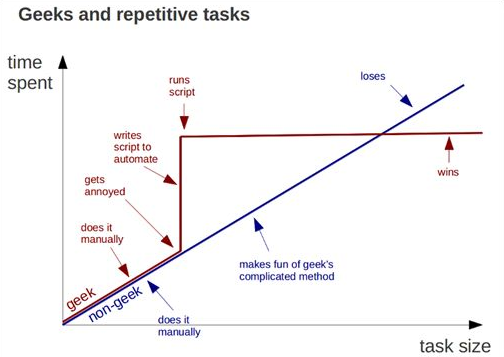
\includegraphics[width=0.9\textwidth]{images/Geeks_and_repetitive_tasks.png}}
    \end{center}
    \caption{Tự động hóa hệ thống bằng kịch bản}
    \label{fig:geeks_and_repetitive_tasks}
\end{figure}

Có rất ít các kịch bản đã được phát triển theo cách đặc biệt này được xuất bản, có tài liệu hay sử dụng lại. Thêm vào đó, bản quyền đối với hầu hết những kịch bản kể trên đều thuộc về những người quản trị hệ thống đã viết ra nó, và thường nó sẽ bị bỏ lại khi họ rời bỏ tổ chức đó hoặc chuyển sang vị trí khác. Điều này dẫn đến việc cùng một công cụ cứ được làm đi làm lại hết lần này đến lần khác. Thậm chí, đôi lúc chỉ đơn giản là điều đó không phù hợp với cách làm việc của người tại nhiệm hoặc người tại nhiệm không thể nắm bắt được những gì người tiền nhiệm đã để lại.

Khi hệ thống được mở rộng, những ứng dụng và kịch bản tùy chỉnh kiểu này hiếm khi phù hợp với môi trường lớn, và họ thường phải gặp phải rất nhiều vấn đề với tính ổn định, sự linh hoạt và các tính năng. Trong môi trường đa nền tảng, những kịch bản như vậy có xu hướng chỉ phù hợp với một nền tảng nhất định, dẫn đến trong các tính huống thực sự cần thiết sẽ phải tạo ra các kịch bản sử dụng cho BSD, một cái khác cho Linux và thậm chí là một cái khác nữa cho Solaris. Thật là tốn công sức và thời gian khi phát triển cũng như duy trì các công cụ như vậy với hy vọng nó sẽ giảm thiểu những công việc nhiêu khê mà bạn phải làm.

Một cách tiếp cận khác đó là mua các công cụ điều hành và quản lý cấu hình như Opsware của HP, CONTROL-M của BMC, Tivoli của IBM hay Unicenter của CA. Những công cụ thương mại này thường gặp phải 2 vấn đề chính đó là giá cả và tính linh hoạt. Đặc biệt là giá cả, nó có thể nhanh chóng trở thành một vấn đề lớn khi bạn sử dụng nhiều hơn các nền tảng và hạ tầng, giá có thể lên rất cao. Trong những hệ thống lớn, chi phí cho giấy phép sử dụng những công cụ như thế có thể lên tới hàng triệu USD.

Tính linh hoạt cũng là một mối quan tâm chính. Các công cụ thương mại thường đóng mã nguồn và giới hạn các tính năng có sẵn của chúng, có nghĩa là nếu bạn muốn mở rộng chúng để có thêm một tùy chỉnh nào đó phù hợp với hệ thống của bạn, bạn cần phải yêu cầu một tính năng mới, và đương nhiên nó có khả năng phải mất một thời gian chờ đợi và  một số khoản chi phí liên quan. Với sự đa dạng về việc triển khai, các nền tảng, các cấu hình và các ứng dụng trong các tổ chức, thật hiếm khi phát hiện bất kỳ công cụ cung cấp khả năng hoàn toàn tùy chỉnh cho phù hợp với môi trường của bạn.

Có một giải pháp thay thế cho cả việc phát triển phần mềm tự thân và phần mềm thương mại. Đó là Phần Mềm Tự Do Mã Nguồn Mở \footnote{Free and Open Source Software (FOSS): \url{https://en.wikipedia.org/wiki/FOSS}}. Các công cụ quản lý cấu hình mã nguồn mở cung cấp cho các tổ chức, doanh nghiệp 2 lợi ích chính sau:

\begin{itemize}
\item Chúng đi kèm mã nguồn nên có thể mở rộng được
\item Chúng là miễn phí!
\end{itemize}

Với các sản phẩm phần mềm nguồn mở, mã nguồn của công cụ trong tầm tay của bạn, cho phép bạn để phát triển cải tiến hoặc điều chỉnh của riêng bạn. Bạn không cần phải chờ đợi cho các nhà cung cấp để thực hiện các chức năng cần thiết hoặc trả tiền cho các tính năng mới hoặc thay đổi. Bạn cũng là một phần của một cộng đồng người sử dụng và phát triển những người chia sẻ một tầm nhìn cho sự phát triển của công cụ. Bạn và tổ chức của bạn có thể lần lượt đóng góp vào tầm nhìn đó. Kết hợp lại, bạn có thể định hình hướng đi của các công cụ bạn đang sử dụng, đem lại thêm sự linh hoạt tổ chức của bạn.

Giá cả là một trong những yếu tố quan trọng đối với việc mua bất kỳ công cụ. Với phần mềm tự do mã nguồn mở, nó không phải là một vấn đề. Bạn không phải trả bất cứ chi phí nào cho phần mềm, thêm vào đó bạn còn có được mã nguồn của nó.

Tất nhiên, chúng ta đều biết chẳng bao giờ có một bữa ăn trưa miễn phí cả, không giống như phần mềm thương mại, phần mềm nguồn mở không đi kèm với bất kỳ sự hỗ trợ đảm bảo nào. Nói như thế không có nghĩa là sự hỗ trợ không có sẵn: Nhiều công cụ mã nguồn mở có cộng đồng lớn và rất năng động, ở đó các thành viên trả lời câu hỏi và cung cấp hỗ trợ thông qua các cơ chế như mailing list, diễn đàn, Wiki hay IRC.\footnote{Các công cụ mã nguồn mở, bao gồm cả Puppet hay Chef, cũng có tổ chức cung cấp các phiên bản thương mại hoặc hỗ trợ cho những công cụ này.}
